% Auto-generated from results/bench_multiclass_ovr_fft_cuda_20260505/multiclass_ovr_fft_cuda_s0.csv
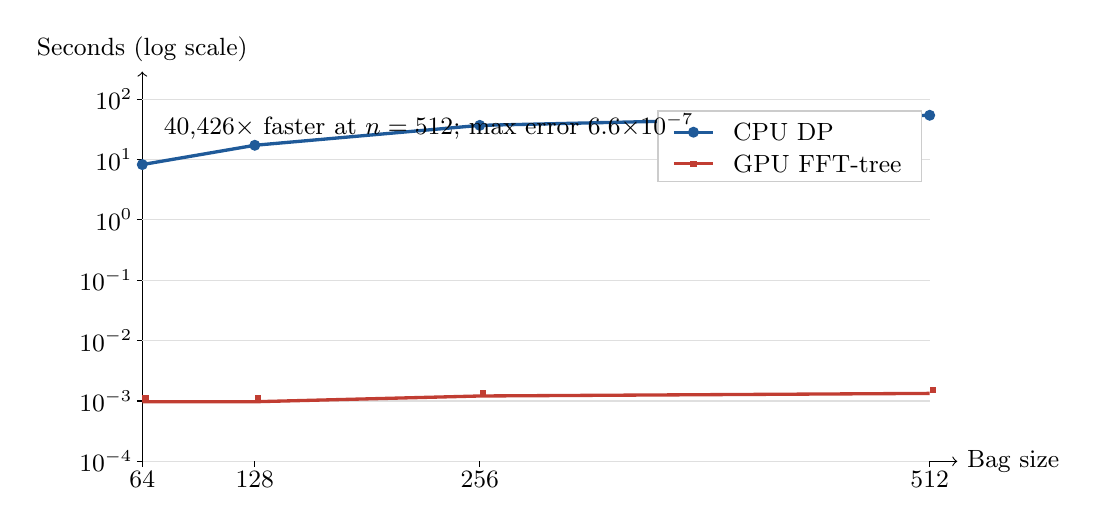
\begin{tikzpicture}[font=\small]
  \definecolor{cpuBlue}{RGB}{31,90,153}
  \definecolor{fftRed}{RGB}{193,61,50}
  \def\plotW{10.0}
  \def\plotH{4.6}
  \draw[->] (0,0) -- (\plotW+0.35,0) node[right] {Bag size};
  \draw[->] (0,0) -- (0,\plotH+0.35) node[above] {Seconds (log scale)};
  \draw[gray!25] (0,0.000) -- (\plotW,0.000);
  \draw (-0.07,0.000) -- (0,0.000) node[left] {$10^{-4}$};
  \draw[gray!25] (0,0.767) -- (\plotW,0.767);
  \draw (-0.07,0.767) -- (0,0.767) node[left] {$10^{-3}$};
  \draw[gray!25] (0,1.533) -- (\plotW,1.533);
  \draw (-0.07,1.533) -- (0,1.533) node[left] {$10^{-2}$};
  \draw[gray!25] (0,2.300) -- (\plotW,2.300);
  \draw (-0.07,2.300) -- (0,2.300) node[left] {$10^{-1}$};
  \draw[gray!25] (0,3.067) -- (\plotW,3.067);
  \draw (-0.07,3.067) -- (0,3.067) node[left] {$10^{0}$};
  \draw[gray!25] (0,3.833) -- (\plotW,3.833);
  \draw (-0.07,3.833) -- (0,3.833) node[left] {$10^{1}$};
  \draw[gray!25] (0,4.600) -- (\plotW,4.600);
  \draw (-0.07,4.600) -- (0,4.600) node[left] {$10^{2}$};
  \draw (0.000,-0.07) -- (0.000,0) node[below] {64};
  \draw (1.429,-0.07) -- (1.429,0) node[below] {128};
  \draw (4.286,-0.07) -- (4.286,0) node[below] {256};
  \draw (10.000,-0.07) -- (10.000,0) node[below] {512};
  \draw[cpuBlue, very thick] (0.000,3.769) -- (1.429,4.014) -- (4.286,4.267) -- (10.000,4.395);
  \fill[cpuBlue] (0.000,3.769) circle (2pt);
  \fill[cpuBlue] (1.429,4.014) circle (2pt);
  \fill[cpuBlue] (4.286,4.267) circle (2pt);
  \fill[cpuBlue] (10.000,4.395) circle (2pt);
  \draw[fftRed, very thick] (0.000,0.757) -- (1.429,0.757) -- (4.286,0.830) -- (10.000,0.863);
  \fill[fftRed] (0.000,0.757) rectangle ++(0.08,0.08);
  \fill[fftRed] (1.429,0.757) rectangle ++(0.08,0.08);
  \fill[fftRed] (4.286,0.830) rectangle ++(0.08,0.08);
  \fill[fftRed] (10.000,0.863) rectangle ++(0.08,0.08);
  \draw[fill=white, draw=gray!40] (6.55,3.55) rectangle (9.9,4.45);
  \draw[cpuBlue, very thick] (6.75,4.18) -- (7.25,4.18); \fill[cpuBlue] (7.00,4.18) circle (2pt);
  \node[anchor=west] at (7.38,4.18) {CPU DP};
  \draw[fftRed, very thick] (6.75,3.78) -- (7.25,3.78); \fill[fftRed] (6.96,3.74) rectangle ++(0.08,0.08);
  \node[anchor=west] at (7.38,3.78) {GPU FFT-tree};
  \node[anchor=west] at (0.15,4.25) {40,426$\times$ faster at $n=512$; max error $6.6{\times}10^{-7}$};
\end{tikzpicture}
